% https://tex.stackexchange.com/a/409577
\documentclass{beamer}
\usepackage{listings}
\usepackage{tikz}
\usepackage{pgfplots}
\lstset{
   language=C++,
   basicstyle=\ttfamily\scriptsize,
   numbers=left,
   captionpos=b
}
\usetikzlibrary{positioning,arrows,tikzmark}
\usetheme{Darmstadt}

\begin{document}

\begin{frame}[fragile]
    \frametitle{Codestructure sample modification}

  \begin{onlyenv}<2>
\begin{lstlisting}[mathescape,escapechar=\%]
// Iterate
for(i = 0 to N-1) {
   %\tikzmark{obbegin}% // Calculate indices
   $\ldots$
   // Calculate coefficient indices
   %\tikzmark{obend}%$\ldots$
   // Evaluate polynomial
   for(j = 0 to 19) {
      if(j == 0) {
         %\tikzmark{ibtarg}%
      }
      $\ldots$
   }
}
\end{lstlisting} 
      \begin{tikzpicture}[overlay, remember picture, thick]
      \draw[decorate,decoration={brace,amplitude=5pt,mirror}] ([shift={(-2pt,6pt)}]pic cs:obbegin) 
         -- ([xshift=-2pt]pic cs:obend) 
            coordinate[midway,xshift=-6pt](Btip);

      \draw[->, rounded corners] (Btip) -- +(-4pt,0) |- (pic cs:ibtarg);
      \end{tikzpicture}
   \end{onlyenv}

\end{frame}

\end{document}
